\documentclass[12pt,a4paper]{article}
\usepackage[utf8]{inputenc}
\usepackage{amsmath}
\usepackage{amsfonts}
\usepackage{amssymb}
\usepackage{graphicx}
\usepackage{amsmath}
\author{Moritz}
\usepackage[left=2cm,right=2cm,top=2cm,bottom=2cm]{geometry}
\begin{document}
\part{Schallgeschwindigkeit in Festkörpern}
\section{Schallgeschwindigkeit in Metall}
\subsection{Versuchsbeschreibung}
Der Elastizitätsmodul ist eine Materialkonstante, die in vielen Bereichen, wie beispielsweise in der Bauphysik, eine wichtige Rolle spielt. Er charakterisiert die relative Längenausdehnung in Abhängigkeit von der angreifenden Zugspannung.
\begin{equation}
E = \dfrac{F/A}{\Delta L/L}
\end{equation}
Da der Elastizitätsmodul für Metall (Größenordnung $10^{11} \dfrac{N}{m^2}$) sehr groß ist, lässt er sich nur für dünne Drähte statisch messen. Für Metallstäbe lässt er sich allerdings über die Mesung der Schallgeschwindigkeit mit Hilfe des Zusammenhangs 
\begin{equation}
v_l = \sqrt{\dfrac{E}{\rho}}
\label{eq:001}
\end{equation}
bestimmen. Ein in der Mitte zwischen zwei Punkten eingespannter Stab der Länge L, Masse M und mit Durchmesser D wird durch geeignetes Anschlagen zu longitudinalen Schwingungen angeregt, wobei für die Grundschwingung $\lambda_0 = 2L$ gilt. Mit der Messung der Frequenz $f_0$ berechnet sich die Schallgeschwindigkeit im Metallstab zu
\begin{equation}
v_l = \lambda_0 \cdot f_0
\label{eq:002}
\end{equation}
und der Elastizitätsmodul zu
\begin{equation}
E = 16 f_0^2 \cdot \dfrac{L M}{\pi D^2}.
\label{eq:003}
\end{equation}
\subsection{Versuchsaufbau}
\begin{figure}
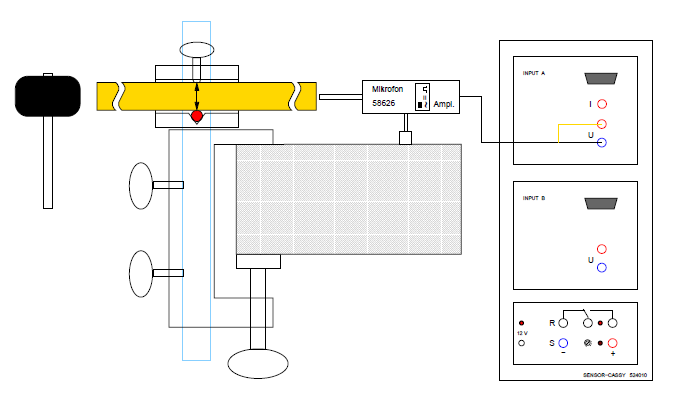
\includegraphics[scale=1]{Bilder/AufbauMessungSchallgeschwindigkeitMetallstab.PNG}
\centering
\caption{Messaufbau Schallgeschwindigkeit in Metallstäben}
\label{StabAufbau}
\end{figure}
Abbildung \ref{StabAufbau} zeigt den mechanischen Aufbau: Der Stab wird mittels einer Kreuzmuffe und einer kurzen Metallstange an einer Tischklemme eingeklemmt. Ein kleiner kurzer Metallstift wird so in die Kreuzmuffe gelegt, dass der Stab nur an zwei gegenüberliegenden Punkten eingeklemmt wird, nämlich zwischen dem Metallstift und der Feststellschraube. Als Messgerät dient ein Mikrofon, welches in ca. 5mm Abstand auf ein Ende des Stabes gerichtet angebracht und an das CASSY angeschlossen wird. 
\subsection{Versuchsdurchführung}
Zunächst müssen die Einstellungen des CASSY angepasst werden. Da die Frequenz der Schwingung bestimmt werden soll, muss die automatische Aufzeichnung verwendet werden. Anhand von Gleichung \eqref{eq:001} lässt sich ersehen, dass die erwarteten Frequenzen sehr hoch sind, daher muss die Intervallzeit im Mikrosekundenbereich ($50 \mu s$) liegen; bei 16000 Messungen liegt die Messdauer dann bei 0,8s. Der Messbereich am CASSY ist nur bedingt relevant, weil sich die Amplitude auch am Mikrofon einstellen lässt. Um Nebeneffekte zu vermeiden, empfiehlt es sich, am CASSY einen mittleren Bereich zu wählen ($|U| \leq 3V$), weil dann auch am Mikrofon ein mittlerer Wert für die Ausgangsamplitude gewählt werden kann. \\

Der Metallstab wird dann mit einem Gummihammer an dem dem Mikrofon abgewandten Ende so angeschlagen, dass die Hammerfläche möglichst parallel zur Stababschlussfläche ist und der Hammerkopf im Moment des Auftreffens nur eine Geschwindigkeitskomponente entlang des Stabes hat. Nach einer sehr kurzen Zeit (Größenordnung 1ms) wird die Messung gestartet. Dadurch wird der Einschwingvorgang in der Messung ignoriert. Dieser Vorgang wird für jeden Stab fünfmal wiederholt. \\

Zuletzt wird der Metallstab ausgemessen und gewogen:
\begin{enumerate}
\item Die Länge L mit dem Bandmaß,
\item den Durchmesser D mit der Mikrometerschraube, gemittelt über fünf Positionen in unterschiedlichen Orientierungen und 
\item die Masse M mit der Analysewaage in drei verschiedenen Orientierungen des Stabes im Raum (Position und Orientierung der Waage bleibt gleich).
\end{enumerate}
\subsection{Versuchsauswertung}
\subsubsection{Rohdaten}
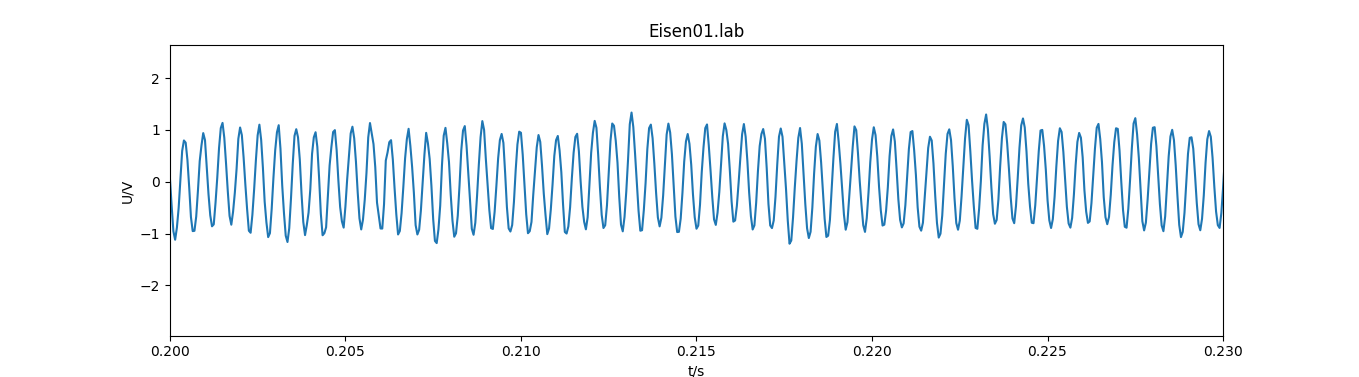
\includegraphics[width=\linewidth,height=\textheight,keepaspectratio]{Bilder/Eisen01.png}
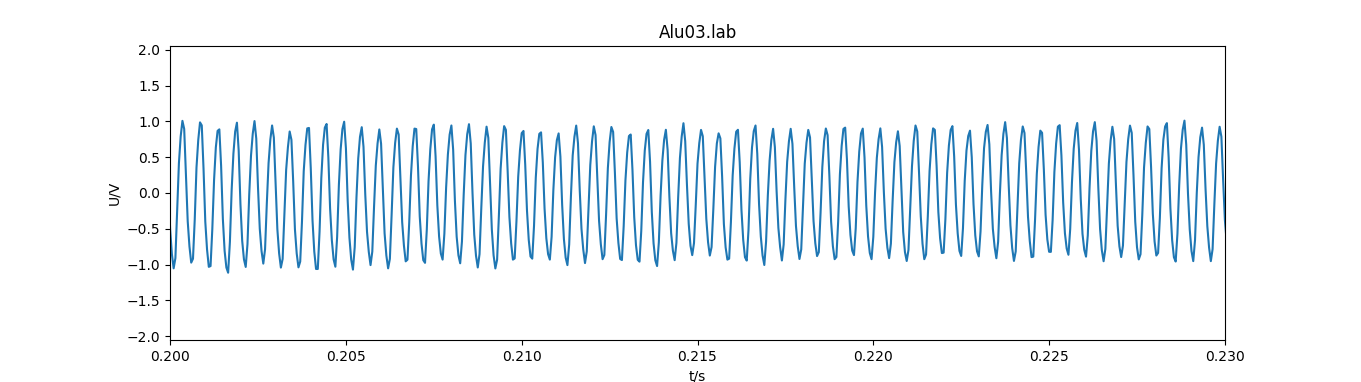
\includegraphics[width=\linewidth,height=\textheight,keepaspectratio]{Bilder/Alu03.png}
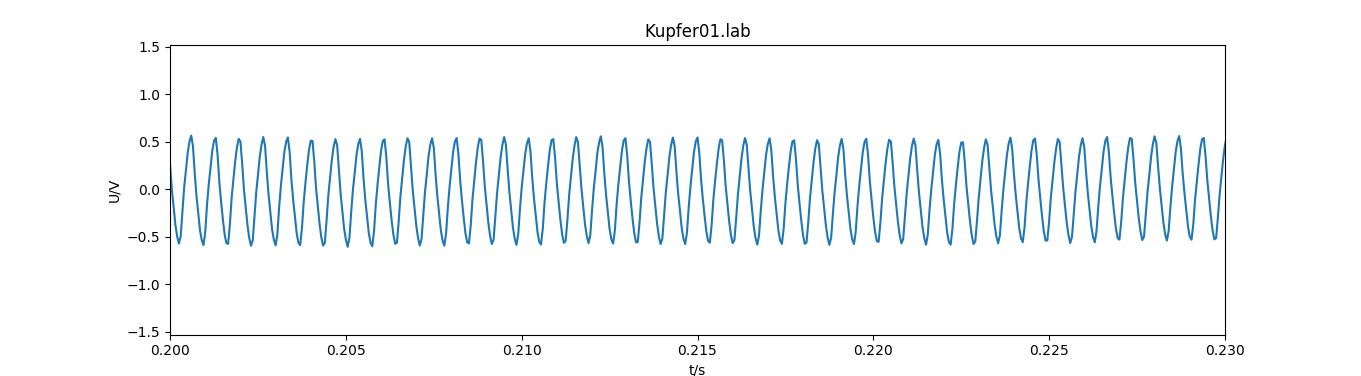
\includegraphics[width=\linewidth,height=\textheight,keepaspectratio]{Bilder/Kupfer01.png}
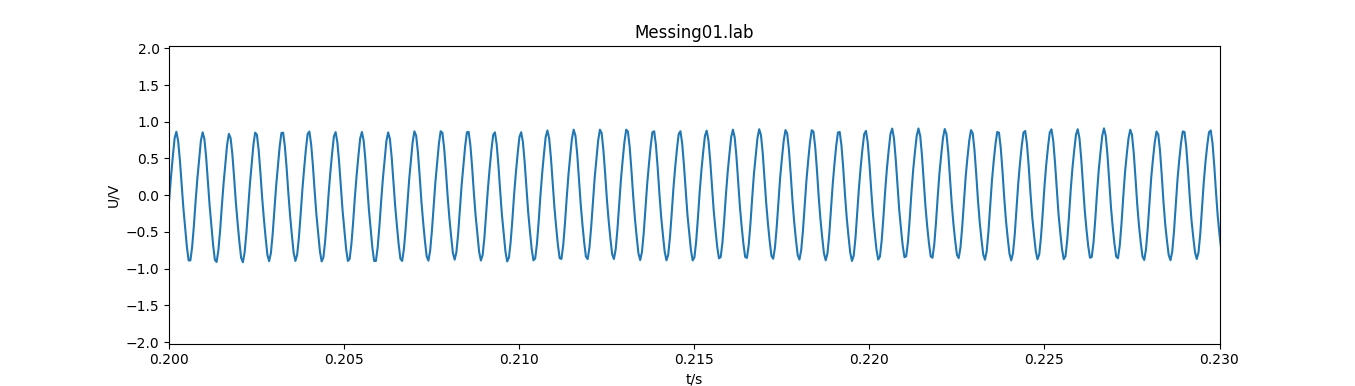
\includegraphics[width=\linewidth,height=\textheight,keepaspectratio]{Bilder/Messing01.png}
\newpage
\subsubsection{Frequenzspektren}
Die Daten wurden mit einer Fast-Fourier-Transformation ausgewertet, da eine normale Fourier-Transformation bei den vorhandenen 20 Datensätzen zu lange gedauert hätte.
Stichproben einer normalen Fourier-Transformation haben aber gezeigt, dass die beiden Methoden nahezu identische Werte ergeben.
Des weiteren wäre eine Bestimmung der Peaklage durch abzählen wegen der hohen Frequenz zu ungenau.\\

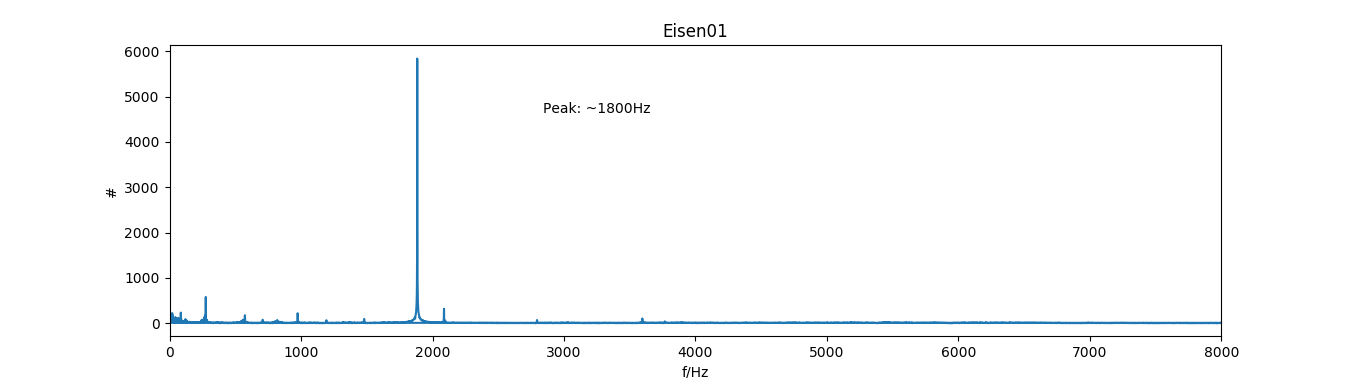
\includegraphics[width=\linewidth,height=\textheight,keepaspectratio]{Bilder/Eisen01_fourier.png}\\
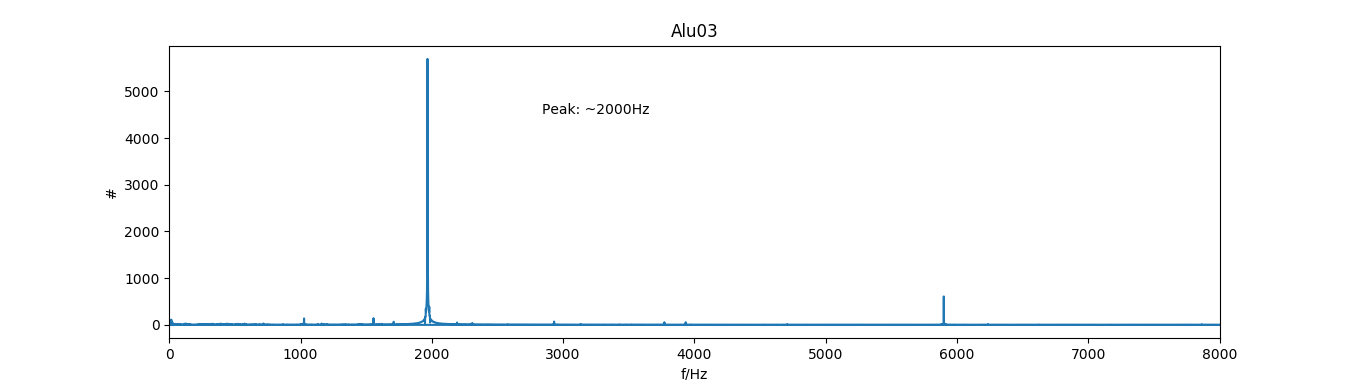
\includegraphics[width=\linewidth,height=\textheight,keepaspectratio]{Bilder/Alu03_fourier.png}\\
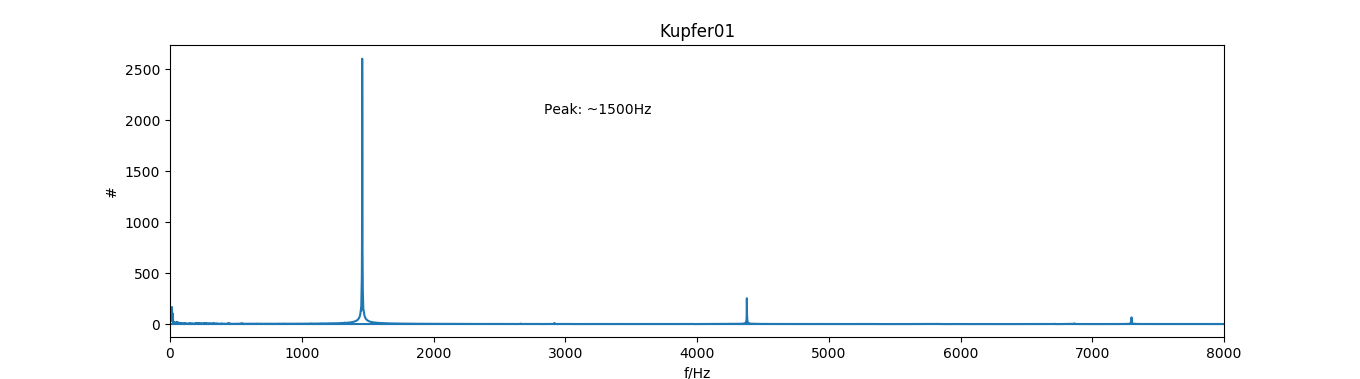
\includegraphics[width=\linewidth,height=\textheight,keepaspectratio]{Bilder/Kupfer01_fourier.png}\\
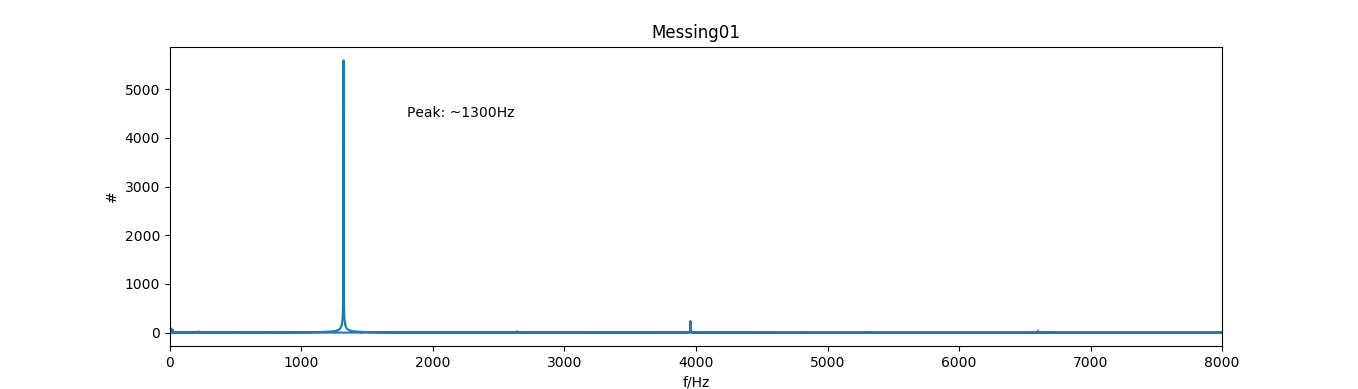
\includegraphics[width=\linewidth,height=\textheight,keepaspectratio]{Bilder/Messing01_fourier.png}\\
Frequenzspektren(von oben nach unten):1.Eisen(Peak:~1800Hz), 2.Aluminium(Peak:~2000Hz), 3.Kupfer(Peak:~1500Hz), 4.Messing(Peak:~1300Hz)
\newpage
\subsubsection{Analyse}
Wegen den Materialeigenschaften der Metalle wir angenommen, dass es sich um Eisen, Aluminium, Kupfer und Messing handelt.
\subsubsection{Ausmessungen}
\begin{tabular}{|c|c|c|c|}
\hline 
Material & Länge[m] & Durchmesser[m] & Masse[kg] \\ 
\hline 
Eisen & $1.303\pm0.0003\pm0.00056$ & $0.01204\pm4.8\cdot10^-5$ & $1.1570\pm1.7\cdot10^-4$ \\ 
\hline 
Aluminium & $1.300\pm0.0003\pm0.00056$ & $0.01199\pm6\cdot10^-5$ & $0.4070\pm6.7\cdot10^-5$ \\ 
\hline 
Kupfer & $1.300\pm0.0003\pm0.00056$ & $0.01195\pm1.8\cdot10^-5$ & $1.2942\pm8.8\cdot10^-5$ \\ 
\hline 
Messing & $1.299\pm0.0003\pm0.00056$ & $0.0119\pm3.7\cdot10^-5$ & $1.2328\pm3.3\cdot10^-5$ \\ 
\hline 
\end{tabular}\\\\
Der statistische Fehler der Länge L ist standardverteilt und beträgt $\sigma_{stat}=\frac{1}{\sqrt{12}}\approx0.3$mm.\\
Der Systematische Fehler ist durch das Maßband mit $0.3+0.2\cdot L$ gegeben. Der Unterschied bei den gemessenen Längen ist minimal, weswegen verallgemeinert $L=1.3m$ und damit $\sigma_{sys}=0.56$mm angegeben wird.\\
Alle anderen Fehler wurden durch Mehrfachmessung aus dem Mittelwert ermittelt.\\
\subsubsection{Ergebnisse der Fourieranalysen}
\begin{tabular}{|c|c|c|c|c|}
\hline 
Material & Eisen & Aluminium & Kupfer & Messing \\ 
\hline 
1.Messung[Hz] & 1883.95 & 1967.00 & 1459.67 & 1321.40 \\ 
\hline 
2.Messung[Hz] & 1884.01 & 1966.96 & 1459.45 & 1321.41 \\ 
\hline 
3.Messung[Hz] & 1884.02 & 1966.93 & 1459.17 & 1321.40 \\ 
\hline 
4.Messung[Hz] & 1884.03 & 1966.60 & 1459.47 & 1321.41 \\ 
\hline 
5.Messung[Hz] & 1884.03 & 1966.58 & 1459.46 & 1321.41 \\ 
\hline 
\end{tabular} 
\\
\\
Daraus folgen die Mittelwerte und der Fehler:\\
Eisen: 		($1884.007\pm0.015$)Hz\\
Aluminium:	($1966.813\pm0.092$)Hz\\
Kupfer:		($1459.406\pm0.058$)Hz\\
Messing:	($1321.407\pm0.002$)Hz\\
\\
Daraus kann man mit den Gleichungen (\ref{eq:002}) und (\ref{eq:003}) die Schallgeschwindigkeit v und das E-Modul E berechnen.\\
Für den Fehler auf v gilt:
\begin{equation}
\sigma_v= v\cdot\sqrt{(\frac{\sigma_L}{L})^2+(\frac{\sigma_f}{f})^2}
\end{equation}
Für den Fehler auf f gilt:
\begin{equation}
\sigma_f=f\cdot\sqrt{(\frac{\sigma_L}{L})^2+2\cdot(\frac{\sigma_f}{f})^2+(\frac{\sigma_M}{M})^2+2\cdot(\frac{\sigma_D}{D})^2}
\end{equation}
\begin{tabular}{|c|c|c|c|}
\hline 
Material  & Frequenz[Hz] & Geschwindigkeit[m/s] & E-Modul[GPa] \\ 
\hline 
Eisen & $1884.007\pm0.015$ & $4909.7\pm1.1\pm2.1$ & $188.0\pm1.1$ \\ 
\hline 
Aluminium & $1966.813\pm0.092$ & $5113.7\pm1.2\pm2.2$ & $72.5\pm0.5$ \\ 
\hline 
Kupfer & $1459.406\pm0.058$ & $3794.5\pm0.9\pm1.6$ & $127.7\pm0.3$ \\ 
\hline 
Messing & $1321.407\pm0.002$ & $3433.0\pm0.8\pm1.5$ & $100.5\pm0.4$ \\ 
\hline 
\end{tabular} 
\\
Hinweis: Die systematische Abweichung auf das E-Modul ist immer kleiner als 0.05 und damit für die Messwerte unwichtig
\newpage
\subsubsection{Vergleich mit Literaturwerten}
Die Literaturwerte sind im allgemeinen für eine Temperatur von 20C angegeben. Die Umgebungstemperatur lag bei 24C. Dieser Unterschied auf die Endwerte ist aber für Festkörper vernachlässigbar.
\begin{table}
\begin{tabular}{|c|c|c|}
\hline 
Material & gemessene Frequenz[Hz] & Literaturwert(long.)[Hz] \\ 
\hline 
Eisen & $4909.7\pm3.2$ & 4910-5170  \\ 
\hline 
Aluminium & $5113.7\pm3.4$ & 5350-6250  \\ 
\hline 
Kupfer & $3794.5\pm2.5$ & 4660 \\ 
\hline 
Messing & $3433.0\pm2.3$ & 3500 \\ 
\hline 
\end{tabular} 
\begin{tabular}{|c|c|c|}
\hline 
Material & gemessenes E-Modul[GPa] & Literaturwert[GPa] \\ 
\hline 
Eisen & $188.0\pm1.1$ & 180-210 \\ 
\hline 
Aluminium & $72.5\pm0.5$ & 70 \\ 
\hline 
Kupfer & $127.7\pm0.3$ & 100-130 \\ 
\hline 
Messing & $100.5\pm0.4$ & 78-123 \\ 
\hline 
\end{tabular} 
\caption{Gemessene Daten und Literaturwerte}
Anmerkung: Für den Wert des E-Moduls von Eisen wurde wegen fehlender Quellen das von Stahl genommen.
\end{table}
\paragraph{Eisen}
Der gemessene Wert für die Geschwindigkeit liegt im Rahmen von einer Standardabweichung im Bereich des Literaturwertes.
Das Elastizitätsmodul stimmt ebenfalls mit dem Literaturwert überein.
\paragraph{Aluminium}
Hier ist die gemessene Geschwindigkeit um 236m/s(70 Standardabweichungen)kleiner als der Literaturwert, das Elastizitätsmodul allerdings um 2.5GPa(5 Standardabweichungen größer)
\paragraph{Kupfer}
Die Geschwindigkeit weicht hier sogar um 866m/s(347 Standardabweichungen) vom Literaturwert ab. Gleichzeitig liegt aber das Elastizitätsmodul im angegebenen Bereich.
\paragraph{Messing}
Die gemessene Geschwindigkeit ist um 67m/s(30 Standardabweichungen) zu klein.
Das Elastizitätsmodul liegt aber wieder im Literatur angegebenen Bereich.
\\\\
Offenbar liegt vor allem bei Aluminium und Kupfer ein sehr großer unbekannter Fehler bei der Geschwindigkeit vor. Es besteht die Möglichkeit, dass die Literaturangaben andere Materialeigenschaften voraussetzen, da die Werte für das Elastizitätsmodul trotz dieses großen Fehlers richtig sind
\newpage


\section{Akustik der Gitarre}
\subsection{Versuchsbeschreibung}
Die Überlagerung zweier Wellen kann mit dem Superpositionsprinzip
\begin{equation}
A(x = 0, t) = \sum_{n=1}^N A_n \cdot \sin (w_nt) \cdot \cos (k_nx) = \sum_{n=1}^N A_n \cdot \sin (w_nt)
\end{equation}
beschrieben werden. Wendet man dieses auf zwei Wellen mit gleicher Amplitude an, lässt sich das Ergebnis mithilfe der Additionstheoreme in einen Term der Form
\begin{equation}
A(x = 0, t) = A_0 \cdot \sin (w_st) \cdot \sin (w_{res}t)
\end{equation}
mit
\begin{equation}
w_s = \dfrac{w_1 - w_2}{2} \quad und \quad w_{res} = \dfrac{w_1 + w_2}{2}
\label{eq:Schwebungsfrequenz}
\end{equation}
umformen. Das wird als Schwebung bezeichnet. Wie sich unschwer erkennen lässt, ist der Schwebungseffekt nur dann hörbar, wenn die beiden ursprünglichen Frequenzen nah beieinander liegen, denn nur dann gilt $w_s \ll w_{res}$. \\
Bei einer Gitarre lässt sich der Ton einer Leersaite mit der nächsthöheren Saite durch Anschlagen bei Verkürzen der Saite am fünften Bund reproduzieren. Wenn nun eine der beiden Saiten leicht verstimmt ist, tritt die Schwebung gut hörbar auf.
\subsection{Versuchsaufbau}
\begin{figure}
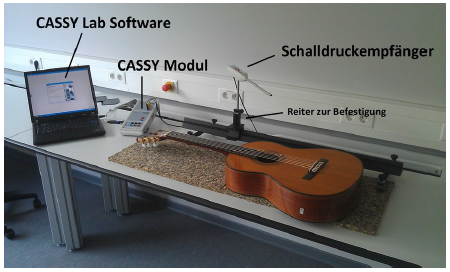
\includegraphics[scale=1]{Bilder/AufbauAkustikGitarre.PNG}
\centering
\caption{Messaufbau Schallgeschwindigkeit in Metallstäben}
\label{GitarreAufbau}
\end{figure}
Die Gitarre wird auf einer dämpfenden Unterlage aufgelegt, um äußere Einflüsse zu minimieren. Das Mikrofon wird in einem Abstand von ca. 25cm über dem Schallloch der Gitarre befestigt und an das CASSY angeschlossen.
\subsection{Versuchsdurchführung}
\label{GitarreEinstellungen}
Zunächst muss die Gitarre gestimmt werden. Dazu wird das Stimmgerät am Gitarrenkopf befestigt und eine Saite unverkürzt angeschlagen. Das Stimmgerät zeigt die ggfs. notwendige Änderung der Saitenspannung an. Dies wird mit allen Saiten wiederholt. Nun wird eine Saite verstimmt. Dazu wird die Saitenspannung um eine halbe Umdrehung der Spannschraube verändert. Der Messbereich am CASSY bleibt im Vergleich zum ersten Versuch unverändert bei $|U| \leq 3V$. Da die Frequenzen einer Gitarre nicht ganz so hoch liegen reicht hier ein Messintervall von $200 \mu s$; bei 16000 Messungen ergibt sich eine Messdauer von 3,2s. \\
Es werden für die Messung immer jeweils die verstimmte Saite am fünften Bund verkürzt und die nächsthöhere Saite angeschlagen. Die Messung wird auch hier wieder mit kurzem Zeitversatz (ca. 20ms) gestartet, um den Einschwingvorgang in der Messung zu ignorieren. Dieser Vorgang wird fünfmal wiederholt.

\subsection{Versuchsauswertung}
\subsubsection{Rohdaten}
\begin{figure}
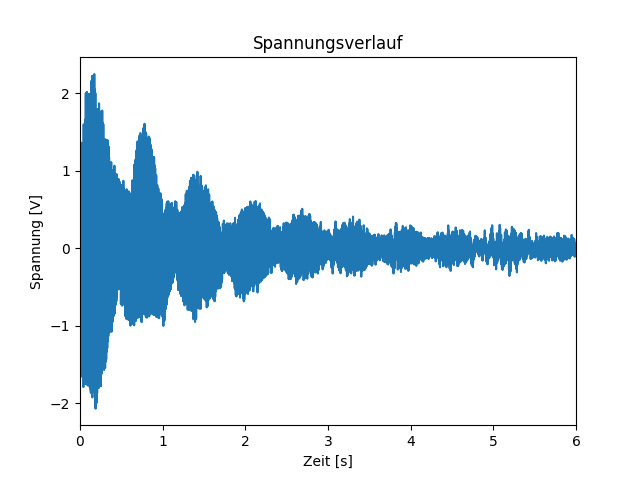
\includegraphics[scale=1]{Bilder/Schwebung_roh.png}
\centering
\caption{Schwingung zweier Gitarrensaite mit nur leicht unterschiedlichen Frequenzen}
\label{Schwebung_roh}
\end{figure}
Die Schwebung ist gut durch die Schwankungen der Amplitude zu erkennen. Die resultierende Frequenz ist nicht direkt ersichtlich, dazu muss in das Bild "reingezoomt" werden. Dabei gerät die Schwebung aus dem Blickfeld.
\begin{figure}
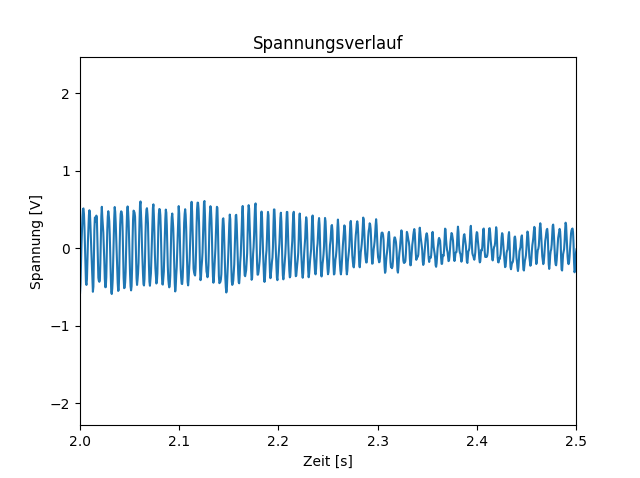
\includegraphics[scale=1]{Bilder/Schwebung_reingezoomt.png}
\centering
\caption{Schwingung zweier Gitarrensaite mit nur leicht unterschiedlichen Frequenzen; kurzes Zeitintervall}
\label{Schwebung_zoom}
\end{figure}
\subsubsection{Frequenzspektren}
Die Schwebungsfrequenz kann nun auf zweierlei Arten bestimmt werden. Möglichkeit eins ist die Berechnung aus den beiden Originalfrequenzen, die mithilfe der Fast-Fourier-Transformation aus den Daten bestimmt werden. Diese liefert für jeden Datensatz ein Frequenzspektrum wie in Abbildung \ref{Schwebung_Frequenzspektrum}. Die Schwebungsfrequenz wird dann mit Gleichung \ref{eq:Schwebungsfrequenz} berechnet. \\
Die zweite Möglichkeit besteht darin, die Schwebungsfrequenz durch Abzählen der Amplitudenminima in den Rohdaten zu bestimmen. Dazu werden alle sichtbaren Amplitudenminima abgezählt und anschließend durch die Differenz der Zeitpunkte des ersten und des letzten Minimums geteilt.
\begin{figure}
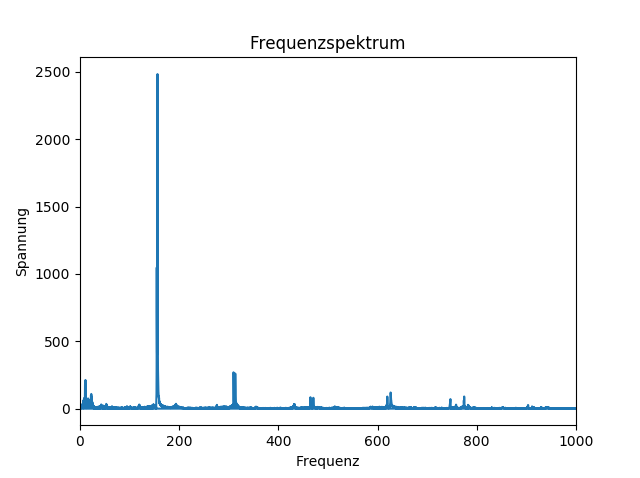
\includegraphics[scale=1]{Bilder/Frequenzspektrum_ges.png}
\centering
\caption{Gesamtes Frequenzspektrum}
\label{Schwebung_Frequenzspektrum}
\end{figure}
Der erste hohe Peak ist zweigeteilt, wie sich bei näherer Betrachtung gut erkennen lässt. Das sind die beiden Saitenfrequenzen (vergleiche Abbildung \ref{Schwebung_zoom}).
\begin{figure}
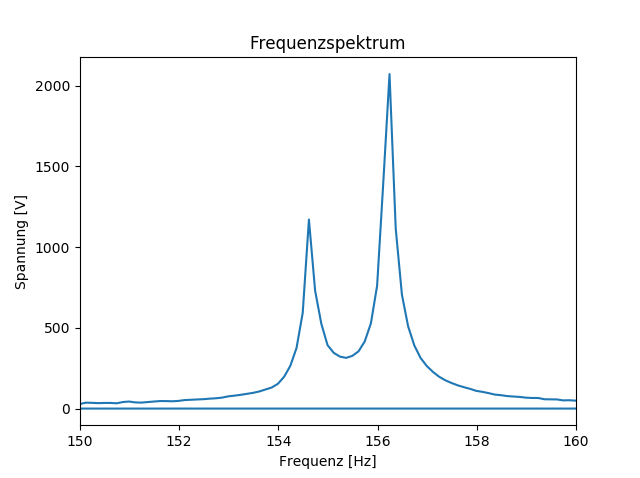
\includegraphics[scale=1]{Bilder/Frequenzspektrum_zoom.png}
\centering
\caption{Ausgeschnittenes Frequenzspektrum}
\label{Schwebung_Frequenzspektrum_zoom}
\end{figure}
\subsubsection{Analyse}
Die beiden beschriebenen Methoden führen zu folgenden Ergebnissen: \\
\begin{tabular}{|c|c|c|}
\hline 
• & Ergebnis der FFT & Wert durch Ablesen \\ 
\hline 
1. Messung & (1.06 $\pm$ 0.36) Hz & (1.60 $\pm$ 0.10) Hz \\ 
\hline 
2. Messung & (1.25 $\pm$ 0.07) Hz & (1.64 $\pm$ 0.10) Hz \\ 
\hline 
3. Messung & (1.75 $\pm$ 0.14) Hz & (1.85 $\pm$ 0.10) Hz \\ 
\hline 
4. Messung & (1.25 $\pm$ 0.14) Hz & (1.61 $\pm$ 0.10) Hz \\ 
\hline 
5. Messung & (1.31 $\pm$ 0.07) Hz & (1.43 $\pm$ 0.10) Hz \\ 
\hline 
\end{tabular} \\
\\Der Fehler auf die Frequenz aus der FFT ergibt sich dabei aus einer Bestimmung der Peak-Breite und der Annahme, dass die Frequenz innerhalb dieses Peaks gleichverteilt ist. Damit berechnet sich dieser für eine Peak-Breite $bp_1$ auf die erste und eine Peak-Breite $bp_2$ auf die zweite Frequenz zu
\begin{equation}
\sigma_f = \dfrac{bp_1 + bp_2}{\sqrt{12}}
\end{equation}
\subsubsection{Auswertung}
Die Ergebnisse aus der FFT und die abgelesenen Werte liegen jeweils zwischen weniger als 1 und knappen 6 Standardabweichungen (aus der FFT) auseinander. Auffällig ist, dass die Werte aus der FFT alle kleiner sind, als die zugehörigen abgelesenen Werte.
\section{Bestimmung der Saitenspannung einer Gitarre}
\subsection{Versuchsbeschreibung}
Eine für die Tonqualität wichtige Eigenschaft einer Saite ist das Verhältnis aus Saitenspannung T zu Massebelag $\mu$. Es gilt der Zusammenhang
\begin{equation}
f_n = \dfrac{n}{2L} \cdot \sqrt{\dfrac{T}{\mu}}.
\label{eq:SpannungMassebelag}
\end{equation}
Dabei ist L die Länger der am Bund verkürzten, frei schwingenden Saite und n charakterisiert, um welche (Ober-)Schwingung es sich handelt. Der Grundton ergibt sich also für $n=1$.
\subsection{Versuchsaufbau}
Der Versuchsaufbau ist identisch zu dem im Kapitel \ref{GitarreAufbau} beschriebenen.
\subsection{Versuchsdurchführung}
Zunächst müssen die Längen der an den Bünden verkürzten Saiten mit dem Maßband gemessen werden. \\
Die Messparameter für Mikrofon und CASSY sind identisch wie in Kapitel \ref{GitarreEinstellungen} beschrieben.
Anschließend wird die Saite angeschlagen und die Messung mit kurzem Zeitversatz (ca. 20ms) gestartet. Diese Messung wird zehnmal wiederholt, wobei jedes Mal die Saite um einen Bund verkürzt wird.
\subsection{Versuchsauswertung}
\subsubsection{Rohdaten}
\begin{figure}
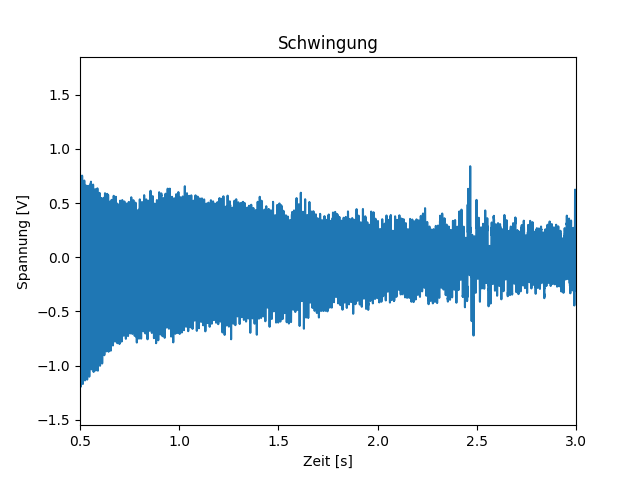
\includegraphics[scale=1]{Bilder/Gitarre_Schwingung.png}
\centering
\caption{Frequenzspektrum einer Gitarrensaite}
\label{Schwingung_Rohdaten}
\end{figure}
Abbildung \ref{Schwingung_Rohdaten} zeigt die Rohdaten. Hieraus lässt sich kaum etwas ablesen, abgesehen davon, dass es sich um eine Schwingung handelt.
\subsubsection{Frequenzspektren}
Wesentlich mehr Aufschluss gibt da das Frequenzspektrum aus der FFT (siehe Abbildung \ref{Saite_Frequenzspektrum}). Hier sind die Grundschwingung (erster Peak) und die Oberschwingungen gut erkennbar, ebenso wie das Abfallen der Amplituden der Peaks mit $A_n \propto \dfrac{1}{n}$.
\begin{figure}
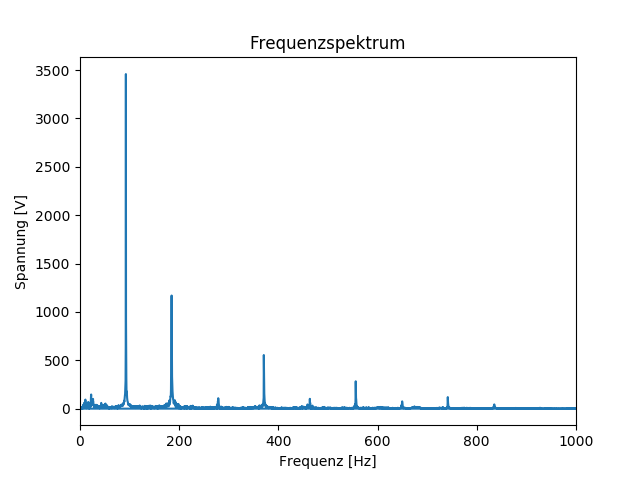
\includegraphics[scale=1]{Bilder/FrequenzspektrumGitarrensaite.png}
\centering
\caption{Frequenzspektrum einer Gitarrensaite}
\label{Saite_Frequenzspektrum}
\end{figure}
\subsubsection{Analyse}
Die aus den Daten mit der FFT ermittelten Frequenzen und die zuvor an der Gitarre gemessenen Saitenlängen finden sich in der Tabelle. \\
\begin{tabular}{|c|c|c|}
\hline 
Bund & Frequenz [Hz] & Länge [m] \\ 
\hline 
1 & 83,75 $\pm$ 0,09 & 0,650 $\pm$ 0,001 \\ 
\hline 
2 & 87,18 $\pm$ 0,27 & 0,616 $\pm$ 0,001 \\ 
\hline 
3 & 92,18 $\pm$ 0,36 & 0,582 $\pm$ 0,001 \\ 
\hline 
4 & 95,93 $\pm$ 0,09 & 0,548 $\pm$ 0,001 \\ 
\hline 
5 & 103,12 $\pm$ 0,09 & 0,516 $\pm$ 0,001 \\ 
\hline 
6 & 106,24 $\pm$ 0,09 & 0,487 $\pm$ 0,001 \\ 
\hline 
7 & 116,24 $\pm$ 0,72 & 0,459 $\pm$ 0,001 \\ 
\hline 
8 & 122,49 $\pm$ 0,81 & 0,434 $\pm$ 0,001 \\ 
\hline 
9 & 129,37 $\pm$ 0,09 & 0,410 $\pm$ 0,001 \\ 
\hline 
10 & 134,99 $\pm$ 0,09 & 0,387 $\pm$ 0,001 \\ 
\hline 
\end{tabular} 
\\Mittels Gleichung \ref{eq:SpannungMassebelag} lässt sich nun eine lineare Regression durch auftragen von $f$ gegen $\dfrac{1}{2L}$ durchführen. Die Steigung der Ausgleichgeraden ist dann die Wurzel aus dem Verhältnis der Saitenspannung zu Massebelag. \\
Führt man dies durch, erhält man folgenden Wert:
\begin{equation}
\sqrt{\dfrac{T}{\mu}} = (98,98 \pm 2,67)\sqrt{\dfrac{Nm}{kg}}
\end{equation}
\subsubsection{Vergleich mit Herstellerangaben}
Der Hersteller hat für die Saite die Werte zu $T = 63,50N$ und $\mu = 5,6712 \cdot 10^{-3} \dfrac{kg}{m}$ angegeben. Damit ergibt sich der "Literaturwert" für die gemessene Größe zu 
\begin{equation}
\sqrt{\dfrac{T}{\mu}} = 105,82 \sqrt{\dfrac{Nm}{kg}}
\end{equation}
Der gemessene Wert liegt also ca. 2,6 Standardabweichungen von den Herstellerangaben entfernt.
\end{document}
